\chapter[Cronograma]{Cronograma}

\section{Trabalho de Conclusão de Curso - Parte 1}

O trabalho teve inicio no segundo semestre de 2013, com o período letivo sendo iniciado em 19 de agosto. A orientação e início das atividades sendo aprovado na segunda semana. 

O trabalho foi realizado com o auxílio do orientador, havendo uma reunião semanal todas as segundas feiras para discussões e análise do projeto. 

Durante as primeiras três semanas do projeto foi realizada uma pesquisa literária para buscar informações sobre o assunto e viabilizar a ideia proposta. Informações sobre literaturas que utilizavam algoritmos procedurais, tecnologias e técnicas utilizadas na área ou ferramentas existentes foram buscadas. 

Na terceira semana de setembro foi construído o primeiro protótipo do sistema, sendo capaz de utilizar dois algoritmos procedurais, parametrizados através da linha de comando, e mostrá-los de forma simples na tela para representação visual e verificação de alterações entre rodadas. 

Na última semana de setembro foi dado ao sistema a capacidade de salvar um mapa em um arquivo e carregar um dado mapa. Ao invés da geração em tempo de compilação. Foi construída uma entidade capaz de se mover através do mapa em áreas classificadas como passáveis. 

Na primeira semana de outubro foi feito a refinação do protótipo, adicionada um sistema de console capaz de realizar comandos simples para auxiliar em testes. Foi também adicionada a visibilidade e descoberta de blocos. A câmera foi ajustada para centrar-se no jogador e foi ajustado o zoom para haver um maior foco. 

Na segunda semana de outubro os gráficos do sistema, antigamente quadrados monocromáticos foram substituídos por imagens simples (16x16 pixels) e foi adicionado suporte a \textit{scripts} lua ao sistema. 
Foi adicionado uma interface para representação de atributos e estados do jogador. Foram também adicionados inimigos e o algoritmo de busca utilizando A* caso jogador estivesse em sua área de detecção. 

Na terceira semana de outubro foi adicionado um simples sistema de ítens, capaz de aumentar os atributos do jogador permanentemente, ou aumentar estados como a sua vida. Foi adicionado também a capacidade de criação de modelos bases para ítens e inimigos através de um arquivo .lua, e a base das métricas foi construída. 

Na quarta semana foram feitos testes relativos a inteligência artificial do BOT e a sua movimentação através de \textit{scripts} .lua. A coleta de algumas métricas também foi realizada. Foi construído a primeira versão da inteligência artificial capaz de encontrar \textit{tiles} e explorar o mapa de forma consistente, porém ainda não otimizada. 

Na primeira semana de novembro foi otimizada a IA para detecção de inimigos e priorização de áreas através da alteração de variáveis. Foi também construído o teste automático de N jogos em M mapas de forma direta, ou seja, sem a influência do jogador, após o inicio da ação. Foram dispostas métricas relacionadas a cada uma das séries de jogos através de médias, desvios padrões e variâncias do número de vezes jogados num dado mapa. 

O restante do mês de novembro foi utilizado como foco na confecção do documento escrito, até a sua data final dia 27/11


\section{Trabalho de Conclusão de Curso - Parte 2}

A segunda parte do trabalho será utilizada para o refinamento e aprimoração da idéia, assim como testes para verificar e estabelecer novas métricas baseados em resultados obtidos de forma real. 

A segunda parte do trabalho será dividida em dezesseis semanas. Apesar de prováveis mudanças, o cronograma esperado é:

\begin{itemize}
\item[1] - Durante a primeira semana será feito uma revisão do trabalho e a formalização o cálculo da análise das métricas finais de qualidade.

\item[2] - Será dado início no protótipo para obtenção das métricas formalizadas através de jogos automatizados. 

\item[3] - Será otimizado o sistema, dando a ele uma melhor interface e apresentação de métricas. 

\item[4] - Será implementado os perfis de BOT e criado a opção para escolhe dos perfis testados. 

\item[5] - Serão feitos ajustes na representação das métricas, permitindo a visualização de detalhes por jogos, métricas e perfis, além da métrica de qualidade geral.

\item[6] - Serão feitos ajustes e considerações de novas métricas e implementação de novos algoritmos procedurais para testar o sistema.

\item[7] - Será adicionado a capacidade de criação de mapas procedurais através de \textit{scripts} .lua e será também criado um simples editor de mapas para confecção manual de mapas.

\item[8] - Serão criados mapas manuais e realização de testes comparativos entre mapas manuais e procedurais. 

\item[9] - Serão realizados testes por usuários humanos para reafirmar métricas e a análise dos resultados obtidos e formalização de novas métricas, caso necessário.

\item[10] - Serão realizados novos testes de usuário utilizando métricas aprimoradas.

\item[11] - Será feita a formalização do sistema e refatoração e ajuste de interface gráfica e representação. 

\item[12-16] - Serão realizados ajustes finais no sistema e a confecção do documento
\end{itemize}

A Figura 17 - \ref{fig17} mostra um diagrama de gantt da realização de acordo com o calendário de aulas de 2014/1. 

\begin{figure}[h]
	\centering
	\label{fig17}
		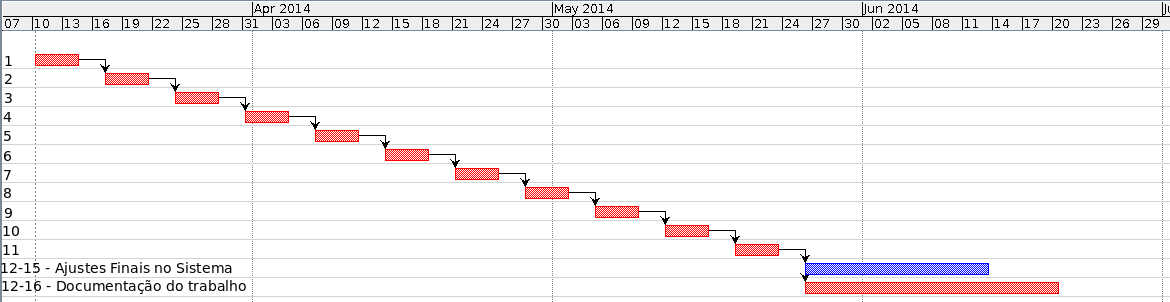
\includegraphics[keepaspectratio=true,scale=0.38]{figuras/fig17-cronograma2v.png}
	\caption{Diagrama de Gantt da segunda etapa do trabalho}
\end{figure} 


\begin{comment}
\begin{figure}[h]
	\centering
	\label{fig17}
		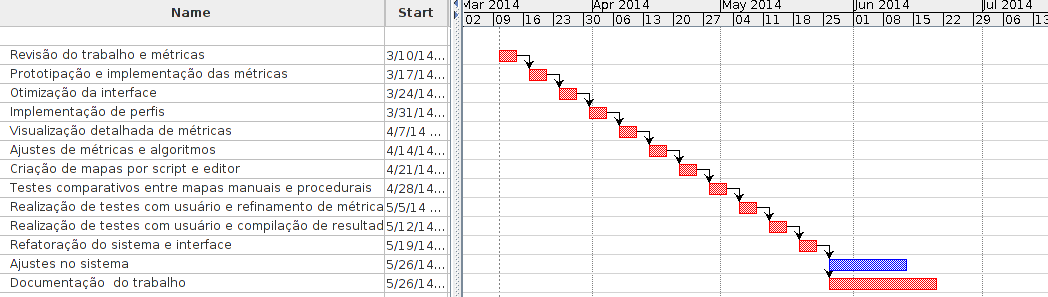
\includegraphics[keepaspectratio=true,scale=0.4]{figuras/fig17-cronograma.png}
	\caption{Diagrama de Gantt da segunda etapa do trabalho}
\end{figure} 
\end{comment}


\chapter{Resultados Alcançados}

	A realização do trabalho até este ponto resultou em um protótipo de parte da ferramenta. O protótipo é capaz de carregar mapas, ítens e inimigos a partir do formato especificado e realizar uma simulação básica de jogos. 
	A ferramenta é capaz de coletar métricas básicas sobre:
\begin{itemize}			
	\item Quantidade de passos;
	\item Inimigos derrotados;
	\item Porcentagem de vitórias;
	\item Dinheiro coletado;
\end{itemize}

	Ainda não é realizada a concretização das métricas em um valor único de qualidade esperada, porém ela gera as médias, desvios padrões e variâncias para medidas de $N$ jogadas em um mesmo mapa. 
	
	O sistema possui um BOT parametrizado com variáveis de ganância com itens, \textit{tiles} solitários e número de iterações extras, podendo ser alterado somente através da modificação dentro do \textit{script} Lua no momento. Não há ainda a diferenciação de perfis por parte do sistema. 
	
	Ítens e inimigos são carregados através de \textit{scripts} Lua, atribuindo-os a um identificador de texto para serem chamados pela função de geração procedural do mapa de forma mais consistente. 
	
	A ferramenta disponibiliza uma simples interface de botões e menus para ajustes de parâmetros para o algoritmo procedural do mapa que será gerado ao iniciar o jogo. É disponibilizado também um botão para carregar um mapa de um arquivo, sem a geração de um novo mapa. 
	
	As devidas condições de vitória e derrota para o jogador estão implementadas, e o sistema possui um console interno que pode ser chamado para alterar propriedades de \textit{debug}, como \textit{setFog} para remoção ou adição de visibilidade, ou \textit{botDelay}, para ajustes na velocidade de processamento do BOT. 
	
	Inimigos estão atacando o jogador quando dentro de sua área de visão e as devidas mensagens de informações são mostradas em uma área na parte de cima da tela como: \lq\lq Você causou 5 de dano ao inimigo\rq\rq.
	
	O sistema está utilizando gráficos 16x16 pixels para representação visual de seus elementos. 
\section{Conclusão}
	O trabalho realizado possibilitou a confirmação da viabilidade da ferramenta e constatou que a necessidade que se tem em obter métricas concretas para mapas gerados automaticamente para acelerar o processo de desenvolvimento de jogos do gênero \textit{roguelike}, é um fator real.	
	
	A definição de diversos perfis de usuário foram observados e classificados para que uma melhor representação das métricas obtidas dos jogos simulados. 
	A ferramenta para a avaliação dos mapas, assim como a forma com que serão testados e extraídas as métricas foram estabelecidas, confirmando-as através da aplicação prática do sistema através de protótipos obtendo a comprovação de que seus conceitos básicos estão funcionando e sendo aplicados. 
	
	O trabalho obteve resultados positivos quanto aos seus benefícios para o desenvolvimento dos jogos, possibilitando a realização de simulações e obtenção de métricas de dezenas de jogos em apenas alguns minutos. 






%CITES
\begin{comment}
\nocite{ArTerrainGen}
\nocite{Decipher}
\nocite{DesAudVid}
\nocite{DesAud}
\nocite{Noel}
\nocite{TaxonomySearchBasePCG}
\nocite{Voronoid}
\nocite{automaticDunGen}
\nocite{contest}
\nocite{pcgwiki}
\nocite{chunsoft}
\nocite{ArTerrainGen}
\nocite{izuna}
\nocite{depthsearch}
\nocite{Astar}
\nocite{normal}
\nocite{montgomery}
\end{comment}